\documentclass{article}%
\usepackage[T1]{fontenc}%
\usepackage[utf8]{inputenc}%
\usepackage{lmodern}%
\usepackage{textcomp}%
\usepackage{lastpage}%
\usepackage[head=40pt,margin=0.5in,bottom=0.6in]{geometry}%
\usepackage{graphicx}%
%
\title{\textbf{El gobierno emite resolución para eliminar los contratos colectivos}}%
\author{ANA DÍAZ | anadiaz@el{-}nacional.com}%
\date{20/11/2018}%
%
\begin{document}%
\normalsize%
\maketitle%
\textbf{URL: }%
http://www.el{-}nacional.com/noticias/economia/gobierno{-}emite{-}resolucion{-}para{-}eliminar{-}los{-}contratos{-}colectivos\_260363\newline%
%
\textbf{Periodico: }%
EN, %
ID: %
260363, %
Seccion: %
Economía\newline%
%
\textbf{Palabras Claves: }%
Economía\newline%
%
\textbf{Derecho: }%
2.3%
, Otros Derechos: %
NO\_TIENE%
, Sub Derechos: %
2.3.4%
\newline%
%
\textbf{EP: }%
NO\newline%
\newline%
%
\textbf{\textit{El sindicalista Orlando Chirino afirma que con la medida se “ratifica la decisión unilateral del Ejecutivo desde el 1° de septiembre de aplanar las tablas salariales”}}%
\newline%
\newline%
%
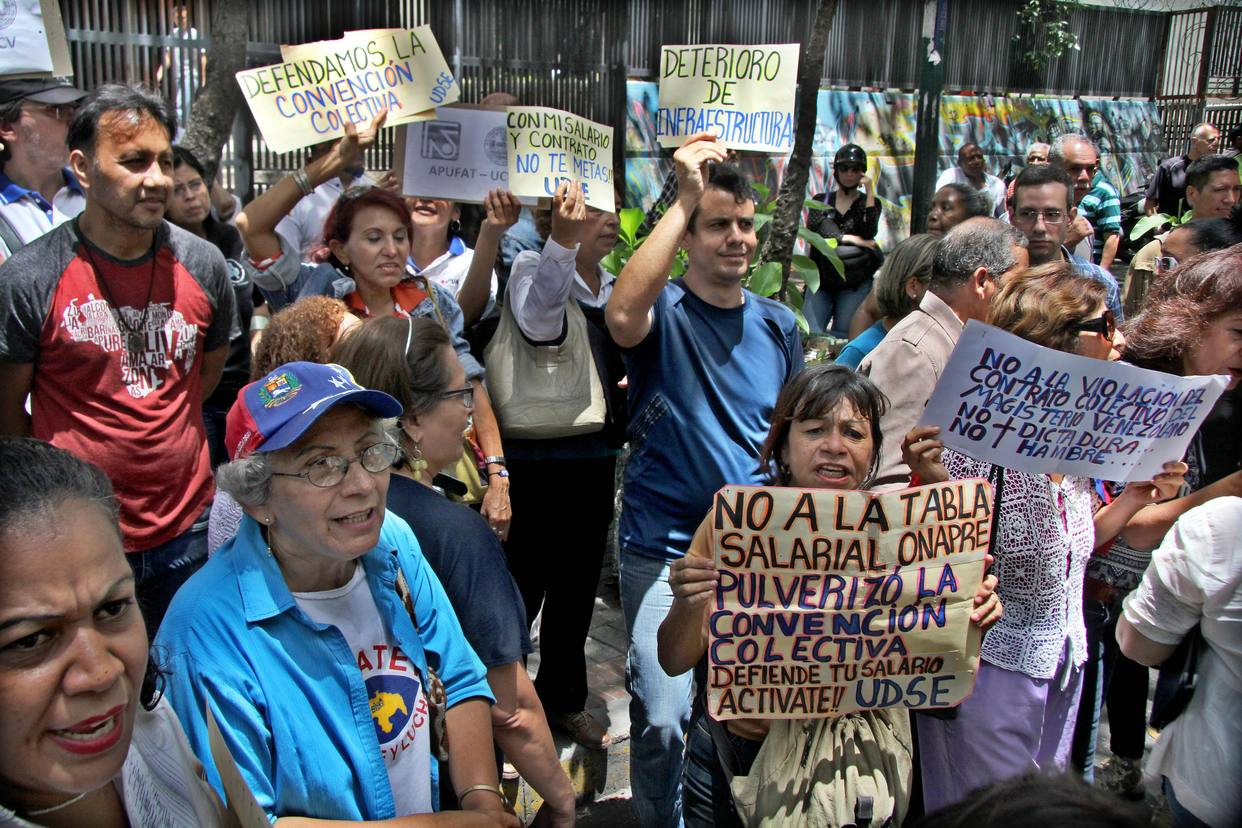
\includegraphics[width=300px]{38.jpg}%
\newline%
%
El gobierno de Nicolás Maduro da otro duro golpe a los derechos de los trabajadores, logrados durante años de lucha, con la resolución 2792 del Ministerio del Trabajo, fechada el 11 de octubre. “La medida establece que los tabuladores tienen como piso un salario mínimo”, advirtió Orlando Chirino, dirigente de Corriente Clasista Unitaria, Revolucionaria y Autónoma.%
\newline%
%
El instructivo, al que se tuvo acceso, indica los lineamientos para las convenciones colectivas y está firmado por Eduardo Piñate, titular del despacho. “El gobierno elimina con esta decisión la esencia de la contratación colectiva de los sectores público y privado”, denunció Chirino.%
\newline%
%
Explicó que fijar como piso de los tabuladores el sueldo mínimo decretado ~por el presidente “ratifica la decisión unilateral del gobierno desde el 1º de septiembre de aplanar las tablas salariales”.%
\newline%
%
El primer nivel de los tabuladores de muchas convenciones colectivas supera un salario mínimo y aunque la resolución señala que se respetará la cláusula de los contratos ya firmados, deja en el limbo qué ocurrirá cuando venzan.%
\newline%
%
“Esto significa que los contratos que están por discutirse o renovarse vuelven al piso de un salario mínimo en contra del principio de la progresividad de los derechos laborales”, sostuvo.%
\newline%
%
La resolución elimina también las instancias laborales de negociación y conciliación entre empleadores y representantes de los trabajadores en los contratos, con la imposición de unas mesas técnicas con funcionarios que están plegados totalmente al Ejecutivo, lo cual lleva a decisiones discrecionales y sesgadas.%
\newline%
%
El sindicalista insistió en que la resolución irrespeta flagrantemente los derechos consagrados en~la Constitución,~la Ley~Orgánica~del Trabajo y~la Organización Internacional~del Trabajo.%
\newline%
%
Agregó que la decisión de Maduro de subir el salario mínimo de~30 a~1.800 bolívares soberanos al mes, desde el 1º de septiembre, es el primer paso para imponer el modelo de Cuba, donde todo el mundo gana lo mismo y no existen las convenciones.%
\newline%
%
El alza salarial fue acompañada del aplanamiento de los tabuladores y la supresión y rebaja de primas y bonos, lo que causó la ola nacional de protestas de sindicatos y trabajadores en las últimas semanas.%
\newline%
%
“Maduro hizo lo que quisiera hacer la economía más liberal del mundo: meter en un solo saco las remuneraciones salariales de todo un país. Con las medidas gubernamentales el trabajador venezolano es el más barato y peor pagado del mundo. En septiembre, con los 1.800 bolívares, ganaba 30 dólares ahora con la inflación es menos de 10 dólares”, dijo Froilán Barrios, coordinador del Frente Autónomo de Defensa del Empleo, el Salario y el Sindicato.%
\newline%
%
Barrios destacó que el gobierno desconoce la antigüedad, la capacitación profesional y técnica, los grados de responsabilidad y la meritocracia de los trabajadores, lo cual desmotiva especialmente a los jóvenes: “¿Para qué estudiar, esforzarse o especializarse si todos ganan lo mismo?”.%
\newline%
%
\end{document}